% -*- root: 00-main.tex -*-
\section{Methods}
\label{sec:methods}
%

\subsection{Susceptibility-derived distortions}
\label{sec:distortions}
\Gls*{dmri} data are usually acquired with \gls*{epi} schemes.
In order to quickly probe the diffusion process within the brain in many different orientations,
  these sequences minimize the bandwidth of the \gls*{pe} direction.
This low bandwidth originates the artifactual displacement of locations presenting small deviations
  from the main magnetic field $B_0$.
One important source of these deviations ($\Delta B_0$) is the discontinuity of magnetic
  susceptibility across the imaged object.
Tissue/air boundaries show large steps of susceptibility and this artifact is
  particularly evident in the surroundings of the orbito-frontal lobe or the temporal
  bone of both hemispheres.
Distortion can be rendered as a registration problem between the undistorted $R$ (reference), 
  and distorted $M$ (moving) spaces:

  \begin{align}
  U_s\colon R \subset \mathbb{R}^n &\to M \subset \mathbb{R}^n \notag\\
  \vec{r} &\mapsto \vec{r}' =\vec{r}+u(\vec{r}),
  \label{eq:transform}
  \end{align}
%
  where $\vec{r}$ denotes a position in $R$, $\vec{r}'$ is
  its corresponding location in $M$, and $n$ the dimensionality of images.
Finally, $\vec{u} = u(\vec{r})$ is the displacement of every point with respect
  to the reference domain.

The displacements field $U_s$ along the \gls*{pe} axis can be estimated theoretically
  \citep{jezzard_correction_1995}:

  \begin{equation}
  \vec{r}' = \vec{r} + \frac{\gamma \, T_{acq}\, s_{PE}}{2\pi}\Delta B_0(\vec{r}) \cdot \hat{\vec{e}}_{PE},
  \label{eq:fieldmap}
  \end{equation}
%
where $\gamma$ is the gyromagnetic ratio, $T_{acq}$ is the readout time,
  $s_{PE}$ is the pixel size along \gls*{pe}, and $\hat{\vec{e}}_{PE}$ the unitary
  vector along \gls*{pe}.
Several methodologies have been proposed to estimate $U_s$ and fix the artifact.
The first solution consisted on estimating $\Delta B_0$ with field mapping
  techniques \citep{andersson_modeling_2001}.
A second family of methods require an extra \gls*{epi} acquisition, but switching
  the \gls*{pe} axis \citep{chiou_simple_2000} or reversing the direction of gradient \gls*{pe}
  increments \citep{cordes_geometric_2000,holland_efficient_2010}.
\cite{kybic_unwarping_2000} proposed nonlinear registration of the \emph{b0}
  image\footnote{The term \emph{b0} refers to one or more images within the
  \gls*{dmri} dataset that are acquired with a null or very low gradient intensity or
   \emph{b}-value.} of the \gls*{dmri} to an undistorted \gls*{t2} image of
   the same subject.
In the following, we will refer to this method as \gls*{t2b}.
Further developments \citep{irfanoglu_susceptibility_2011} extended the \gls*{t2b} 
  approach to the 3D problem.
Therefore, a typical protocol for the extraction of structural connectivity
  comprehends \gls*{dmri}, \gls*{t1}, and the acquisition determined by the correction
  method of choice \citep{daducci_connectome_2012}.


\subsection{Our method and contributions}
\label{sec:contributions}
%
\emph{Regseg} can be viewed as a derivation of \emph{bbregister} \citep{greve_accurate_2009}.
Both methods exploit the anatomically correct and precise surfaces that are readily
  extracted with \emph{FreeSurfer} \citep{fischl_freesurfer_2012}, mapping them
  to a target \gls*{dmri} image using active contours.
We implemented active contours without edges \citep{chan_active_2001}, that allow
  \emph{regseg} to segment homogeneous regions within the brain, while \emph{bbregister}
  use active contours with edges to look for intensity boundaries in the target image.
Another identifying difference is the deformation model:
  \emph{bbregister} includes an affine transformation and overcomes the distortion
  problem by excluding typically affected regions from computation.
Conversely, \emph{regseg} implements a free-deformation field supported with B-Spline
  functions.
Our method is close to \citep{guyader_combined_2011} and \citep{gorthi_active_2011}
  in the use of active contours without edges for registration, however we avoided
  the use of level sets with the application of shape gradients
  \citep{besson_dream2s_2003,herbulot_segmentation_2006}.
\cite{gorthi_active_2011} used a gaussian regularizer, and \cite{guyader_combined_2011}
  proposed a nonlinear elasticity smoother.
In contrast, \emph{regseg} implements the anisotropic regularization proposed by
  \citep{nagel_investigation_1986}.
We also present an ellaborated evaluation instrumentation to create realistic distortions
  and test algorithms.
Integrating \emph{regseg} and an in-house implementation of the \gls*{t2b} correction
  in the workflow, we compared the performance of both solutions.


\subsection{Cost-function derivation}\label{sec:methods_map}
%
In a Bayesian framework, the mappings $U$ in \eqref{eq:transform} are
  evaluated based on their posterior probability given the observed data
  $R$.
Using the Bayes' rule, the posterior likelihood is computed as:

  \begin{equation}
  P(U \mid R,\Gamma_{l,m}) = \frac{P(R \mid U,\Gamma_{l,m})\, P(U)}{P(R)},
  \label{eq:bayes_rule}
  \end{equation}
%
  where $P(R \mid U,\Gamma_{l,m})$ is the data-likelihood, and
  $\Gamma_{l,m}$ are a set of surfaces corresponding to the interfaces
  between piecewise smooth regions $\Omega_i$, such that
  $\Gamma_{l,m} = \partial \Omega_l \cap \partial \Omega_m$ is the
  contour between competing regions $\Omega_l$ and $\Omega_m$.
The best estimate $\hat{U}$ then fulfills the maximum a posteriori criterium
  \citep{bishop_pattern_2006}, and aligns $\Gamma$ into $R$.

First, we assume independence between pixels, and thus break down the
  global data likelihood into a product of pixel-wise conditional probabilities:

  \begin{equation}
  P(R \mid U,\Omega) = \underset{l}{\prod} \underset{\vec{r}\in \Omega_l}{\prod}
    P\left( \vec{f}' \mid U \right),
  \label{eq:bayes_aposteriori}
  \end{equation}
%
  where $\vec{f}' = R(\vec{r}')$ is the feature vector at the displaced
  position $\vec{r}'$ \eqref{eq:transform} in the multispectral target
  volume.
For convenience, and because it has been shown to be an appropriate approximation
  \citep{leemput_automated_1999,cuadra_comparison_2005}, we introduce two assumptions for each
  region $\Omega_l$:
  1) the features are i.i.d.; and 2) they can be modeled by multivariate normal
  distributions with parameters $\lbrace \boldsymbol{\mu}_l, \boldsymbol{\Sigma}_{l} \rbrace$
  for each region $\Omega_l$.
We then insert the normal distribution into \eqref{eq:bayes_rule} to obtain the full
  formulation of the \emph{data term} of our registration model:

 	\begin{align}
  P( R \mid U, \Omega ) &= \underset{l}{\prod} \underset{\vec{r} \in \Omega_l}{\prod}
  \mathcal{N} ( \vec{f} \mid \boldsymbol{\mu}_l, \boldsymbol{\Sigma}_{l} ) \notag\\
  &= \underset{l}{\prod} \underset{\vec{r} \in \Omega_l}{\prod} \frac{1}{ \sqrt{(2\pi)^{C}\,\left|\boldsymbol{\Sigma}_{l}\right|}}\,{e^{\left(-\frac{1}{2}
  \mdist{f'}{l} \right)}},
  \label{eq:pdf}
  \end{align}
%
  using $\mdist{f}{l}$ to denote the squared \emph{Mahalanobis distance} of $\vec{f}$ with respect
  to the descriptors of region $l$ as
  $\mdist{f}{l} = (\vec{f} - \boldsymbol{\mu}_l)^T \, {\boldsymbol{\Sigma}_l}^{-1} \, (\vec{f} - \boldsymbol{\mu}_l)$.


The smoothness of the resulting displacements field is induced by a Thikonov regularization
  prior:

  \begin{align*}
  P(U) = \underset{\vec{r}}{\prod}\, p(\vec{u}) &=
  \underset{\vec{r}}{\prod}\, p_0(\vec{u}) \, p_1(\vec{u}), \\
  p_0(\vec{u}) &= \mathcal{N}( \vec{u} \mid 0, \mathbf{A}^{-1}), \notag\\
  p_1(\vec{u}) &= \mathcal{N}(  \nabla \vec{u} \mid 0, \mathbf{B}^{-1}),
  \end{align*}
%
  imposing that the distortion and its gradient have zero
  mean and variance governed by the matrices $\mathbf{A} = (a_{ij})$ and $\mathbf{B} = (b_{ij})$.
Since the anisotropy is generally aligned with the imaging axes, $\mathbf{A}$ and $\mathbf{B}$
  can be simplified to diagonal matrices.
For convenience, we will set $\alpha_i = a_{ii}^2$ and $\beta_i = b_{ii}^2$, what can be reduced
  using the Hadamard square root notation\footnote{The Hadamard power of a matrix or a vector
  is the power of its elements $\mathbf{M}^{\circ p} = ({m_{ij}}^{p})$} as
  $\mathbf{A}=\boldsymbol{\alpha}^{\circ\frac12}\,\vec{I}_n$ and
  $\mathbf{B}=\boldsymbol{\beta}^{\circ\frac12}\,\vec{I}_n$.


Finally, the maximum a posteriori problem is adapted into a variational one where we look for
  the minimum of an energy functional, by applying a log-transform:

  \begin{align}
  E(R \mid U) &= -\log \underset{l}{\prod}
  \underset{\vec{r} \in \Omega_l}{\prod}
  \mathcal{N} \left( \vec{f}' \mid \Theta_l \right)\,p_0( \vec{u})\,p_1( \vec{u}) \notag\\
  &= C + \underset{l}{\sum} \int_{\Omega_l}
  \mdist{f'}{l} \,d\vec{r} \notag\\
  &+ \int_{\Omega} \left[ \boldsymbol{\alpha} \cdot \vec{u}^{\circ2}
  + \boldsymbol{\beta} \cdot (\nabla \vec{u})^{\circ2} \right] \,d\vec{r},
  \label{eq:energy}
  \end{align}
%
  this expression is dual to the energy functional corresponding
  to a discrete \gls*{acwe} framework \citep{chan_active_2001}
  with the corresponding anisotropic regularization term \citep{nagel_investigation_1986}.


\subsection{Numerical Implementation}
\label{sec:numerical_implementation}

\begin{figure}
	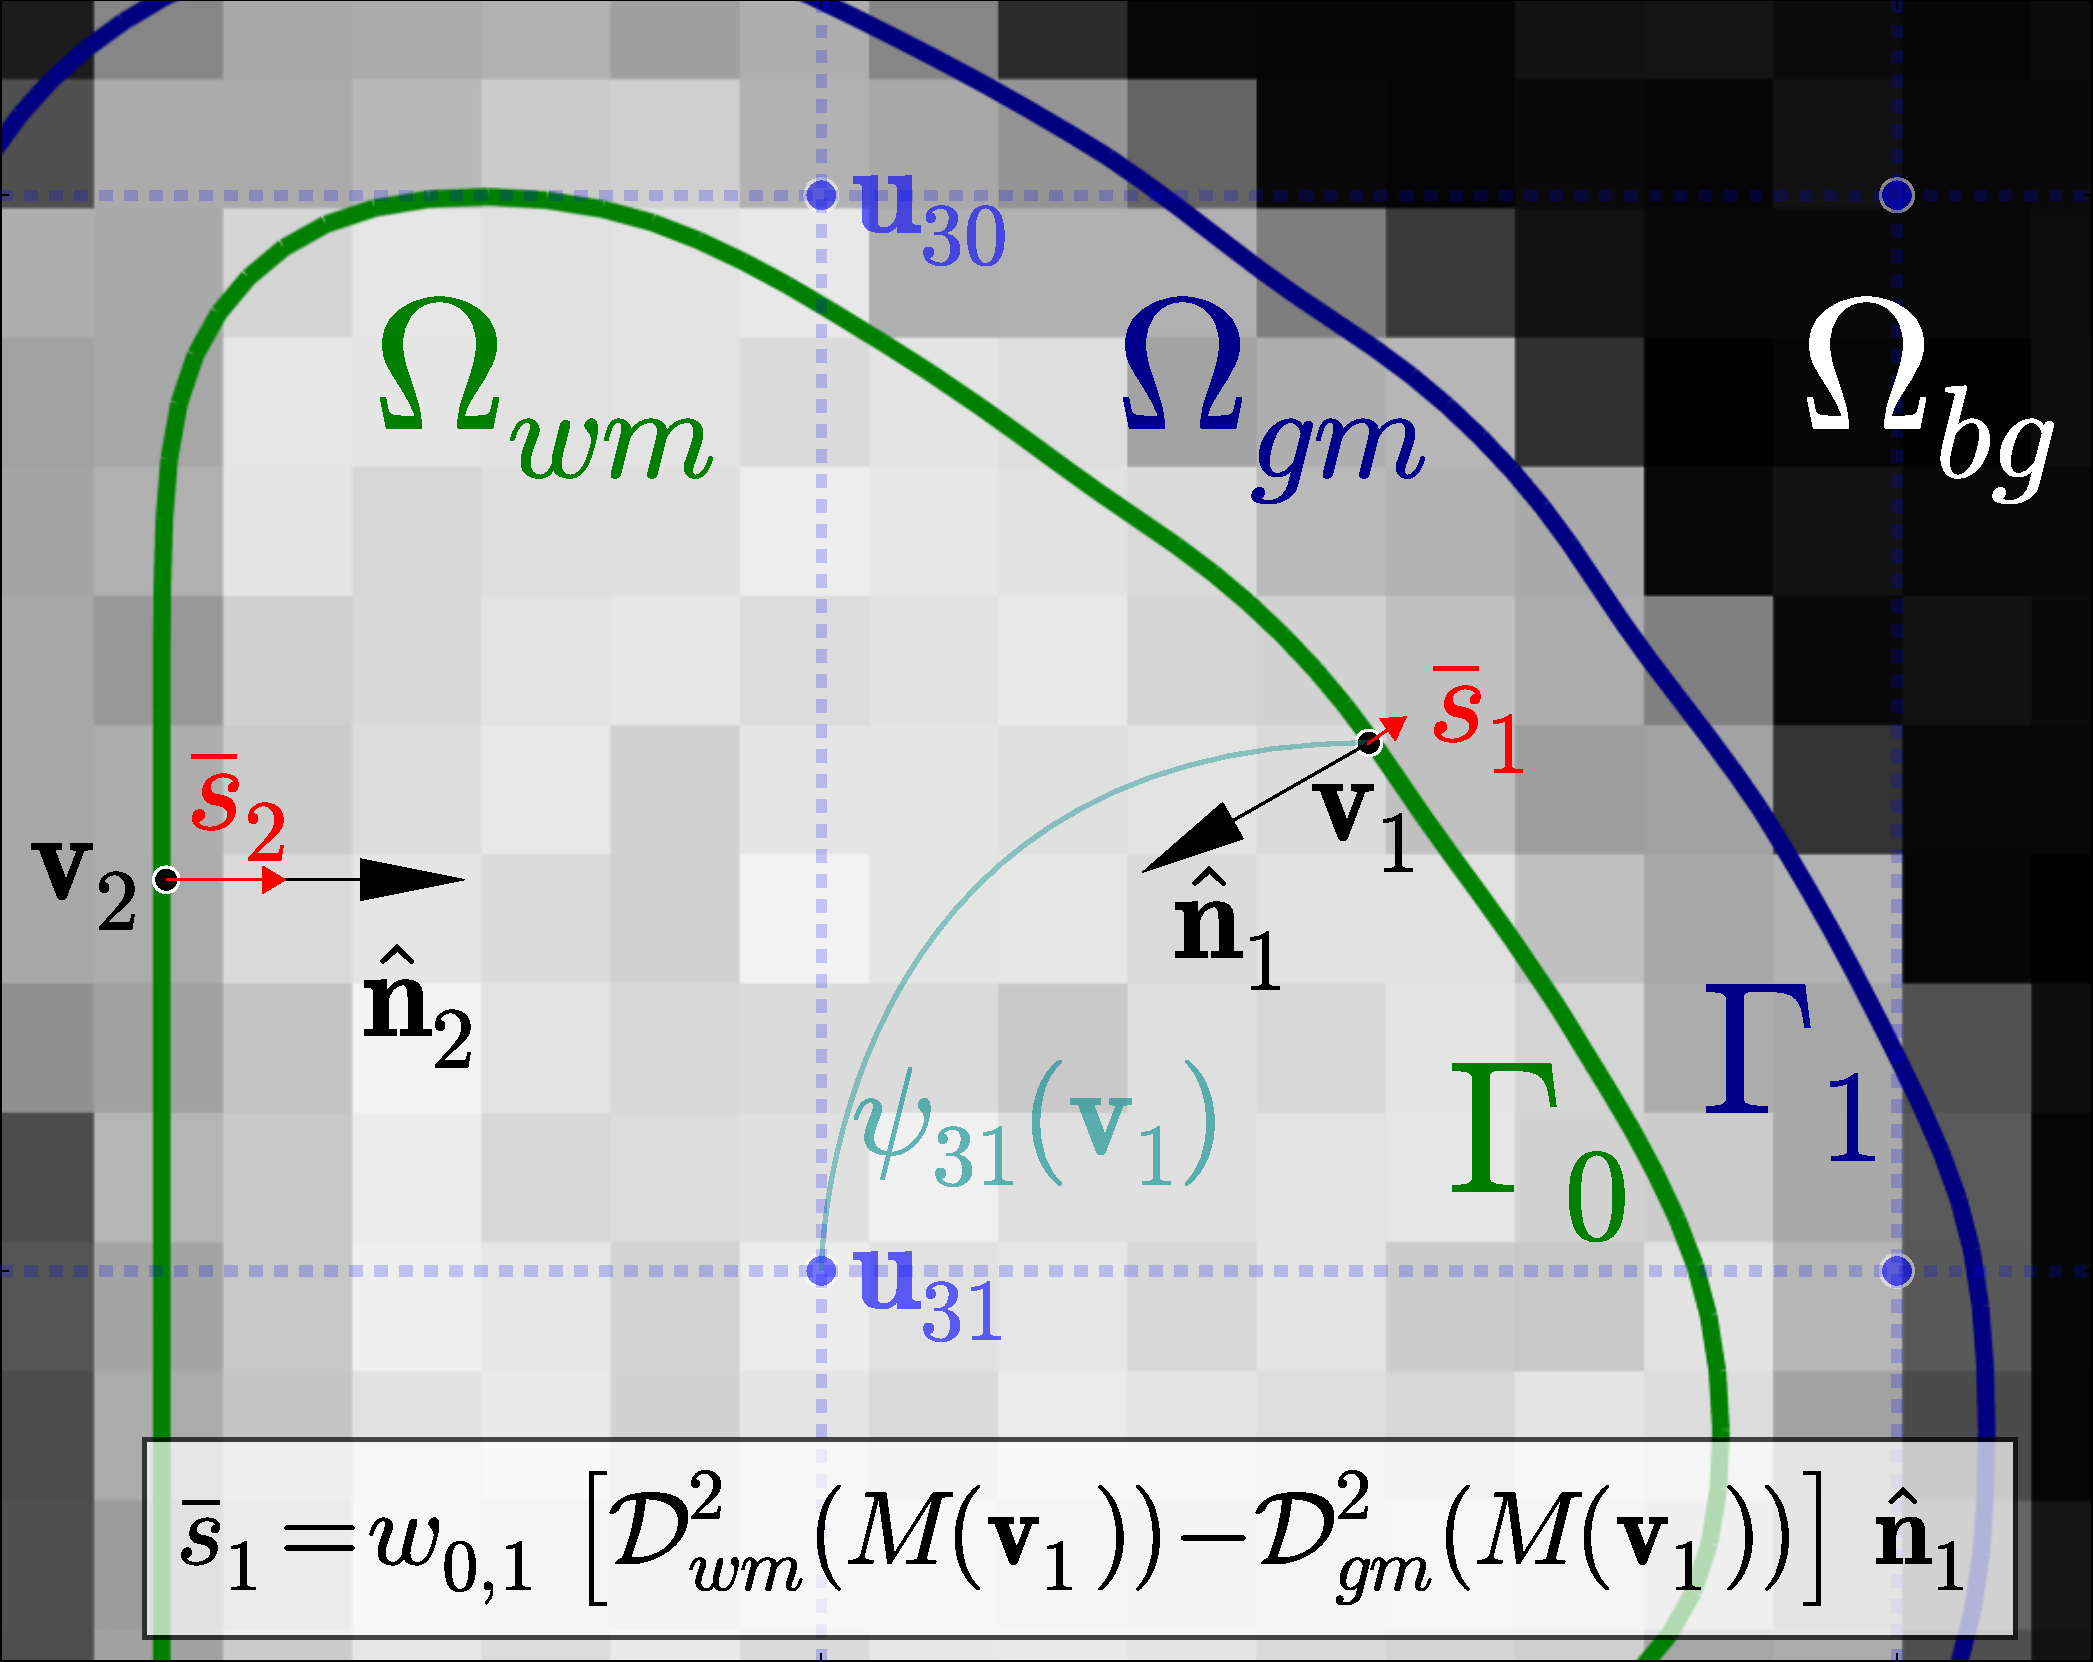
\includegraphics[width=\linewidth]{figures/figure01}
	\caption{The active contours are defined as the interfacing surfaces of the competing
	  \glspl{roi} $\Omega_i$.
	They are represented in green and dark blue colors in this close-up.
	They iteratively evolve following their inner normals $\hat{n}_i$ at each vertex
	  $\vec{v}_i$ of the mesh.
	The gradient speeds $\bar{s}_i$ are computed as the disparity between data energies of
	  the vertex $\vec{v}_i$ in each limiting region (see \ref{app:shape_priors}).
	In this figure, the gradient speed corresponding to $\vec{v}_1$ is written in the lower
	  box, $\Omega_{wm}$ being the inner limiting region and $\Omega_{gm}$ the outer.
	Finally, every $\bar{s}_i$ is associated with the control points $\vec{u}_k$ through
	  the corresponding weights $\psi_k(\vec{v}_i)$ by Eq. \eqref{eq:gradient_wshape}.
	}\label{fig:method}
\end{figure}

\paragraph*{Deformation model}\label{sec:deformation_model}
Let us denote $\{\vec{v}_i\}_{i=1 \ldots N_c}$ the vertices of one or several prior
  surface(s).
In our application, these surfaces are triangularized meshes extracted using \emph{FreeSurfer}
  \citep{fischl_freesurfer_2012}.
The transform $\hat{U}$ \eqref{eq:transform} is supported by a dense deformation field
  $\vec{u} = u(\vec{r})$, such that:

  \begin{equation}
  \vec{v}_i' = \hat{U}\{\vec{v}_i\} = \vec{v}_i + u(\vec{v}_i) = \vec{v}_i + \vec{u}_i.
  \label{eq:nodes_tfm}
  \end{equation}

Since the nodes of the anatomical surfaces likely lay off-grid, it is required to
  derive $u(\vec{r})$ from a discrete set of parameters $\{\vec{u}_k\}_{k=1 \ldots K}$.
Densification is achieved through a set of associated basis functions $\psi_k$:

  \begin{equation}
  u(\vec{r}) = \sum_k \psi_k(\vec{r}) \vec{u}_k.
  \label{eq:intp_kernel}
  \end{equation}

In our implementation, $\psi_k$ is chosen to be a tensor-product B-Spline kernel
  of degree 3 ($\beta_3$).
Then, introducing \eqref{eq:intp_kernel} into \eqref{eq:nodes_tfm} and replacing
  $\psi$ by the actual kernel function, the transformation writes:

  \begin{equation}
    \vec{v}_i' = \vec{v}_i + \sum_k \left[ \vec{u}_k \, \underset{d}{\prod}
      \beta_3( (\vec{v}_i - \vec{r}_k) \cdot \hat{\mathbf{e}}_d ) \right],
  \label{eq:transformation}
  \end{equation}
%
  with $\hat{\mathbf{e}}_d$ being the unitary vector along axis $d$.


\paragraph*{Optimization}
\label{sec:gradient_descent}
To find the minimum of the energy functional \eqref{eq:energy},
  we propose a gradient-descent approach with respect to the underlying
  deformation field through the following \gls*{pde}:

  \begin{equation}
  \frac{\partial u(\vec{r},t)}{\partial t} \propto - \frac{\partial E(R \mid U)}{\partial \vec{u}_k},
  \label{eq:general_gradient_descent}
  \end{equation}
%
  with $t$ being an artificial time parameter of the contour
  evolution, and $\vec{u}_k$ the parameters supporting the estimate
  $\hat{U}$ of the transformation at the current time point.
Now, we introduce \eqref{eq:energy} in \eqref{eq:general_gradient_descent}:

  \begin{align}
  \frac{\partial E(\vec{u})}{\partial \vec{u}_k} &=
  \frac{ \partial }{\partial \vec{u}_k} \Big\{
  \underset{l}{\sum} \int_{\Omega_l} \mdist{f'}{l} \,d\vec{r} \notag\\
  &+ \int_{\Omega} [ \boldsymbol{\alpha} \cdot \vec{u}^{\circ2}
  + \boldsymbol{\beta} \cdot (\nabla \vec{u})^{\circ2} ] \,d\vec{r}
  \Big\}.
  \label{eq:gradient_descent}
  \end{align}


We apply a discretized interpretation of \eqref{eq:shape_gradients} to compute
  the data term in \eqref{eq:gradient_descent} using shape-gradients
  \citep{herbulot_segmentation_2006}, and ultimately avoid level sets.
We refer the reader to the appendix \autoref{app:shape_priors} in order to fill in the gap
  between \eqref{eq:gradient_descent} and the following expression:

  \begin{align}
  \frac{\partial E_{data}(\vec{u})}{\partial \vec{u}_k} &=
  \frac{ \partial }{\partial \vec{u}_k} \left\{
   \underset{\vec{x} \in \Omega_l}{\sum} \underset{l}{\sum} \mdist{f'}{l} \right\} \notag\\
  &= \underset{i}{\sum} w_i
   \left\langle \frac{\partial \vec{v}_i'}{\partial \vec{u}_k}, \bar{s}_i'\right\rangle,
  \label{eq:gradient_wshape}
  \end{align}
%
  in this case, the formulation has been adapted to the non-binary case, $\{l,m\}$
    being any pair of neighboring regions, and $\Gamma_{l,m}$ the contour separating
    them such that
    $\vec{x}' = \vec{v}' \in\Gamma_{l,m} \iff \vec{x}\in \partial\Omega_i \cap \partial\Omega_j$,
    $\bar{s}_i'$ is the speed vector projected on to the unit inward normal to the contour
    at $c_i'$ (described in \autoref{fig:method}), $w_i$ is the area contribution of vertex
    $c_i'$ to the the total area of the surface it belongs.


Finally, we can compute:

  \begin{align}
  \frac{\partial \vec{v}_i'}{\partial \vec{u}_k} &= \frac{\partial}{\partial \vec{u}_k}
  \left\{ \vec{v}_i + \sum_k \psi_k(\vec{v}_i) \vec{u}_k \right\}
  = \psi_k(\vec{v}_i)\, \hat{\vec{e}}
  \label{eq:basis_derivative}
  \end{align}
%
  where $\hat{\vec{e}}$ is the coordinates system's unit vector.
The vertex speeds $\bar{s}_i'$ obtained by computing the shape-gradients \eqref{eq:shape_gradients},
	are then projected to the deformation field in order to obtain the derivatives $\vec{g}_k$
	corresponding to $\vec{u}_k$:

  \begin{equation}
  \vec{g}_{i,k} = w_i \, \left\langle \frac{\partial}{\partial \vec{u}_k}{\vec{v}_i}', \bar{s}_i'\right\rangle
  = - w_i \left[ \mdist{f_i'}{l} - \mdist{f_i'}{m} \right] \psi_k(\vec{v}_i)\, \hat{\vec{n}}_i,
  \end{equation}
%
  then the full gradient evolution equation \eqref{eq:gradient_descent} yields:

  \begin{align}
  \frac{\partial E(\vec{u}_k)}{\partial \vec{u}_k} =
  &\underset{i}{\sum} \vec{g}_{i,k} +2\, \boldsymbol{\alpha} \vec{u}_k
  -2\, \boldsymbol{\beta} \Delta \vec{u}_k,
  \label{eq:gradient_final}
  \end{align}

Finally, we introduce a step size parameter $\delta$ to discretize the artificial time parameter
  in the iterative optimization.
Then, applying the Fourier transform as detailed in the \suppl{section S1}, the
  update equation is derived from \eqref{eq:gradient_final}:

  \begin{align}
  \vec{u}_k^{t+1} = \mathcal{F}^{-1}\left\{ \frac{\mathcal{F}\{\vec{u}_k^t / \delta - \sum_i \vec{g}_{i,k}\}}%
                  {\mathcal{F}\{(1/\delta+\boldsymbol{\alpha})I-\boldsymbol{\beta}\Delta\}} \right\}
  \label{eq:update_equation}
  \end{align}


\paragraph*{Settings, implementation details, and convergence}
\label{sec:conv_report}
The registration parameters (such as $\delta$, $\boldsymbol{\alpha}$, $\boldsymbol{\beta}$,
  the B-Spline grid resolutions, target image smoothing, etc.)
  and other implementation details (for instance the sparse matrix approach
  to fast interpolation) are discussed in the \suppl{section S1}.
The actual choices of parameter settings are publicly distributed with the source code of the experiments.
Additionally, we release our software along with a tool for generating convergence reports to
  demonstrate the behavior of \emph{regseg} and help scientists configure their own experiments.
One sample report is found in the \suppl{section S1.3}.


\subsection{Experiments and evaluation}
\label{sec:experiments_evaluation}
%
In order to demonstrate the performance of \emph{regseg}, we first conducted a battery of
  accuracy tests over synthetic data, and then applied it in the susceptibility distortion
  correction of real data.
\autoref{fig:evworkflows} presents the workflow implementing the evaluation instruments.
Besides a visual assessment of the results, we report quantitative evaluations using
  two metrics.
In the case of the phantoms, since we had produced distortions along the three
  available dimensions, we computed the Haussdorf distance, by reusing the
  ``point-to-cell'' method of \cite{commandeur_vtk_2011}.
Conversely, the susceptibility-derived distortions only happen along the \gls*{pe}
  axis of the image.
Therefore, a \gls*{swindex} can be computed as the one-to-one distance between corresponding
  vertices of surfaces, weighted by their respective Voronoi area $a_i$:

  \begin{equation}
  sWI = \frac{1}{P} \sum\limits_p^P \frac{1}{A_p} \sum\limits_i^{N_p} a_i\,\|
  \vec{v}_i - \hat{\vec{v}}_i \|
  \label{eq:swindex}
  \end{equation}
%
  where $\vec{v}_i$ are the locations of the $N_p$ vertices in each $p \in \{1, \dots P\}$
  prior, $A_p$ the total area of surface $p$, and $\hat{\vec{v}}_i$ is the location
  recovered corresponding to the vertex $\vec{v}_i$.


\begin{figure*}
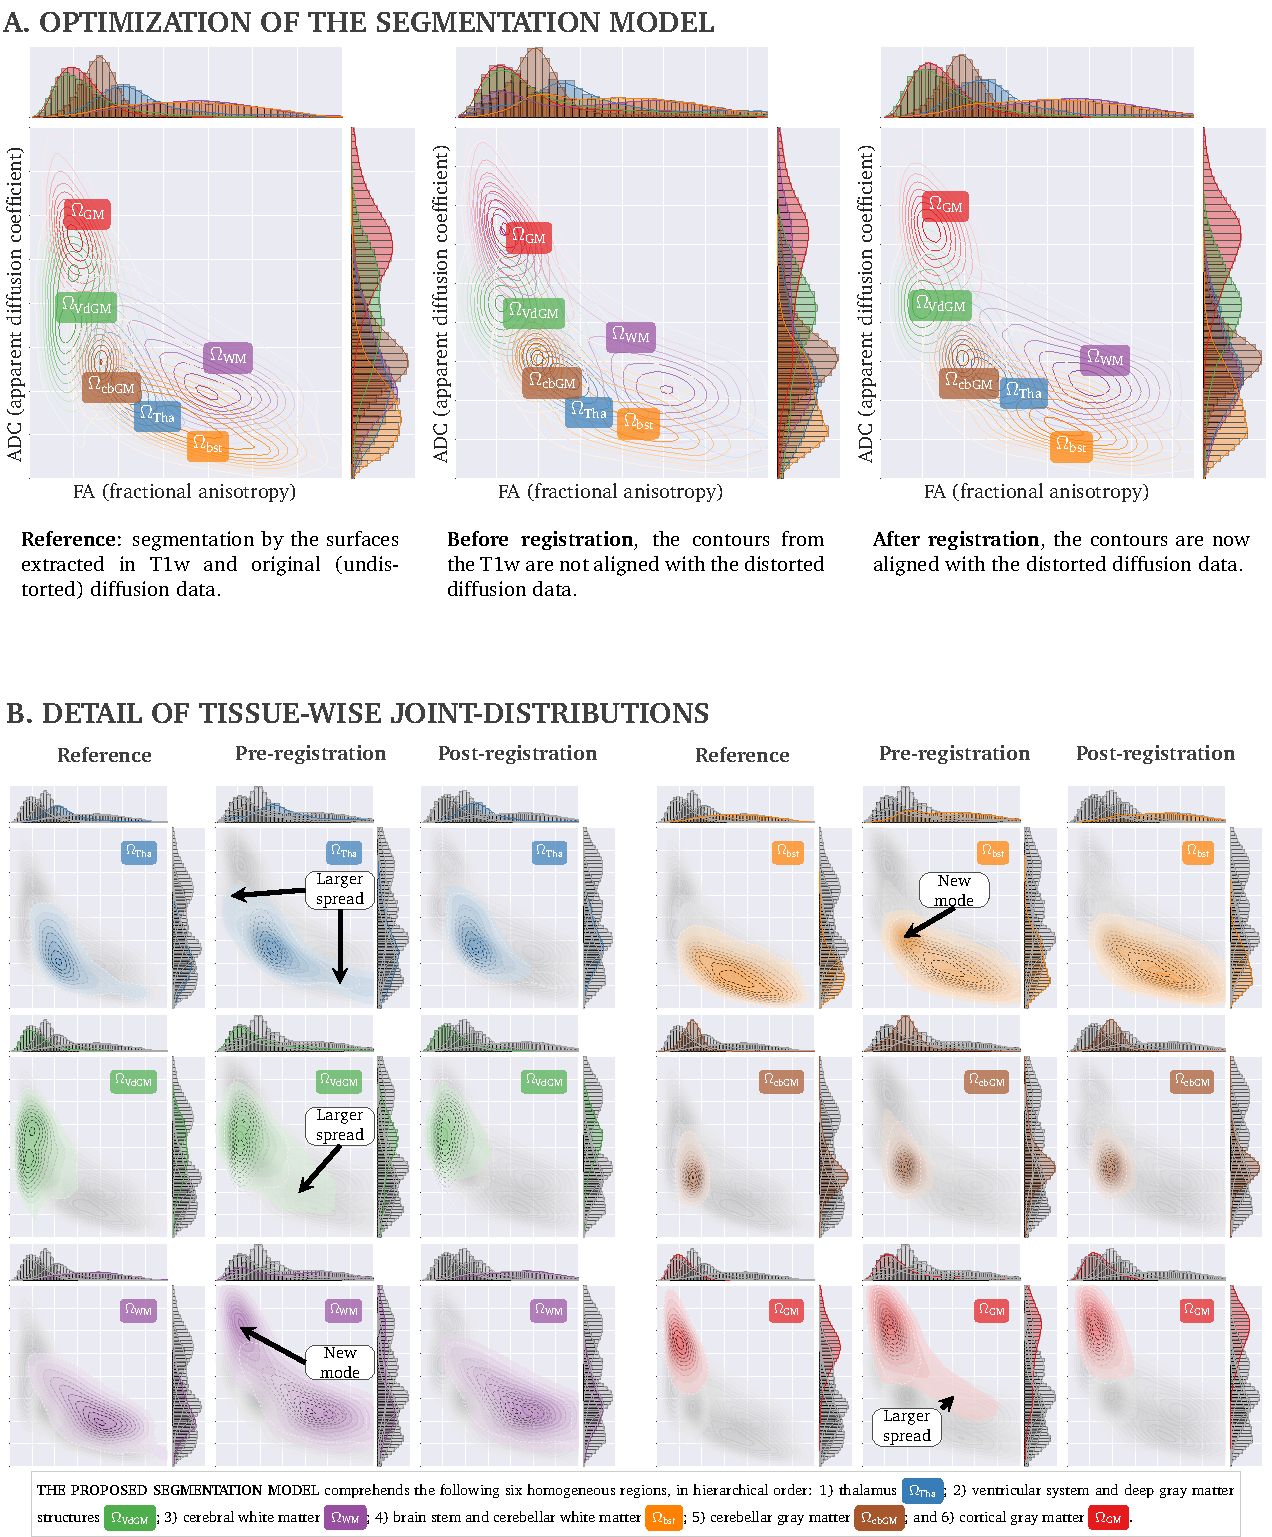
\includegraphics[width=\linewidth]{figures/figure02}
\caption{Experimental workflow applied on real data from the \acrfull*{hcp}.
  1) The prior surfaces are extracted from the anatomical reference (\gls*{t1} image).
	2) To operate as ground truth, we generate a plausible-synthetic distortion $U_{true}$
	  from the fieldmap using \eqref{eq:fieldmap}.
	3) The \gls*{dmri} data are warped using $U^{-1}_{true}$ to reproduce the effects of real
	  susceptibility-derived distortions.
	Target diffusion scalars (\gls*{fa} and \gls*{adc}) are computed on the distorted data and
		stacked to feed the multivariate input required by our algorithm.
	4) \emph{Regseg} is run, obtaining a $U_{test} = \hat{U}_{true}$, the estimation of
	  the ground-truth deformation.
	5) Results are visually and quantitatively evaluated.}\label{fig:evworkflows}
\end{figure*}


\subsection{Image Data and preprocessing}
\label{sec:datasets}

\paragraph*{Simulated phantoms}%
\label{sec:digital_phantoms}
We proved the concept on simplistic digital phantoms which we will name after their
  appearance as ``box'', ``ball'', ``L-shape'', and ``gyrus'' (\autoref{fig:phantom},
  boxes A and B).
Using \emph{phantomas} \citep{caruyer_phantomas_2014}, we simulated
  \gls*{t1} (TE/TR=10/1500ms) and \gls*{t2} images (TE/TR=90/5000ms)
  corresponding to each phantom type, with two resolutions each
  ($1.0mm$ and $2.0mm$ isotropic).
Simulations were corrupted with rician noise for a \gls*{snr} of 300.0.
The reference surfaces were extracted at the higher resolution (1.0mm isotropic),
  using \texttt{mri\_tessellate}\footnote{A marching-cubes algorithm shipped with 
  \emph{FreeSurfer}.}.

\begin{figure*}
    \centering
    \resizebox{\textwidth}{!}{%
      \begin{tikzpicture}
        \node[inner sep=5pt, draw=black!40](fig03a) at (0,14)
          {\includegraphics[width=\linewidth]{figures/figure03-a}};
        \node[inner sep=5pt, draw=black!40](fig03b) at (0,7.6)
          {\includegraphics[width=\linewidth]{figures/figure03-b}};
        \node[inner sep=5pt, draw=black!40](fig03c) at (0,0)
          {\includegraphics[width=\linewidth]{figures/figure03-c}};
        \node[circle, text=black!75] at (-8.8,16.2) {\Huge \textbf{A}};
        \node[circle, text=black!75] at (-8.8,10.05) {\Huge \textbf{B}};
        \node[circle, text=black!75] at (-8.8,3.4) {\Huge \textbf{C}};
      \end{tikzpicture}
    }%
	\caption{A. The ``cortex'' phantom is a spherical shape with two sulci and an
	  outer crust resembling the cortical folding (left).
	The model is used to generate \gls*{t1} and \gls*{t2} images after warping the
	  contours using a random and plausible transformation $U_{true}^{-1}$ (right).
	B. Visual assessment of the results on the low resolution sets:
	  ``gyrus'' (top-left), ``L-shape'' (top-right), ``ball'' (bottom-left),
	  and ``box'' at (bottom-right).
	In yellow color, the recovered contours after registration are represented.
	Our method showed high accuracy, as demonstrates almost exact location of the registered
    contours with respect to their ground truth position depicted in green.
	Partial volume effect turns segmentation of the sulci a challenging problem with voxel-wise
	  clustering methods, but it is successfully segmented with our method.
	C. Quantitative evaluation of registration error in terms of average Hausdorff distance of
	  surfaces at high (left) and low (right) resolutions, demonstrating that the error is
	  consistently below the voxel size.
	  }\label{fig:phantom}
\end{figure*}

To warp the simulated datasets, we generated 150 different realizations of
  the distortion $U_{true}$.
Smoothness is introduced using two levels of B-Spline functions, with control points evenly
  located in isotropic grids covering the full extent of the phantom.
The first level had $50.5mm$ of separation between control points and the second $25.25mm$.
The rationale behind this choice is producing large deformations on the contours with
  the first level, and matching the properties of susceptibility-derived distortions
  as previously reported by \cite{irfanoglu_susceptibility_2011} with the finer grid.
The coefficients of the B-Spline functions were randomly generated for each resolution level.
Invertibility of $U_{true}$ is ensured by controlling the maximum displacement at each
  level ($20.2mm$ and $10.1mm$ respectively) as studied in \citep{rueckert_diffeomorphic_2006}.

\paragraph*{Real datasets} %
\label{sec:human_connectome}
%
For the evaluation of the algorithm on real \gls*{dmri} data of human brains,
  we collected 16 datasets from the ``minimally preprocessed''
	 database of the \gls*{hcp}.
We refer the reader to \citep{essen_human_2012} for exact details about acquisition
  parameters, and \citep{glasser_minimal_2013} for the preprocessing issues.
The datasets comprehend a large set of images, containing \gls*{t1}, \gls*{t2} and
  multi-shell \gls*{dmri} images.
The original acquisitions are released within ``unprocessed'' packages, and
  the ``minimally preprocessed'' are corrected for artifacts, brain-extracted
  and spatially normalized, along with some results of the standard processing
  pipeline of \emph{FreeSurfer}.

Selecting the appropriate labels in the \emph{aparc} segmentation, we applied
  \texttt{mri\_tessellate} to extract the surface of the following
  six homogeneous regions $\Omega_l$:
  1) the thalamus, $\Gamma_{Tha}$;
  2) \gls*{csf} of the ventricular system and deep \gls*{gm} structures, $\Gamma_{VdGM}$;
  3) cerebral \gls*{wm}, $\Gamma_{WM}$;
  4) brain stem and cerebellar \gls*{wm}, $\Gamma_{bst}$;
	5) cerebellar \gls*{gm}, $\Gamma_{cbGM}$; and
	6) cortical \gls*{gm} surface, $\Gamma_{pial}$.
The choice of this particular model is further addressed in \autoref{sec:res_model_and_metric}.

In this case, we derived the deformation $U_{true}$ from the field maps released with
  the corresponding packages of each dataset from the \gls*{hcp} applying \eqref{eq:fieldmap},
  mimicking the real distortions, using a derivation of our previous work
  \citep{esteban_simulationbased_2014}.
After warping the original \gls*{dmri} with $U_{true}^{-1}$, we computed the \gls*{dti} and
  the derived scalars (\gls*{fa} and \gls*{adc}) using \emph{MRtrix} \citep{tournier_mrtrix_2012}.
The stack of \gls*{fa} and \gls*{adc} conforms the multivariate input for \emph{regseg}.

A dual workflow to the general evaluation framework (\autoref{fig:evworkflows})
  was also implemented to integrate the \gls*{t2b} registration scheme.
We reproduced the solution and settings provided with \emph{ExploreDTI}
  \citep{leemans_exploredti_2009}, a widely used toolkit for tractography analysis of
  \gls*{dti}.
\emph{ExploreDTI}, internally uses \emph{elastix} \citep{klein_elastix_2010} to
  perform registration.
First, the average \emph{b0} volume is computed using all the \emph{low-b} volumes within
  the distorted \gls*{dmri} dataset.
Using the ``preprocessed'' instance of the \gls*{t2} image of the corresponding subject as
  reference image, and the \emph{b0} image as moving image, we registered both and
  projected the correct (undistorted) contours to the warped space using the resulting
  transform.